\section{Serial and parallel algorithms performance} \label{s:results:performance-serial-parallel}
	Performance of the parallel algorithms can be measured using different definitions and laws. Figures \ref{fig:speedup:crank-nicolson}, \ref{fig:speedup:explicit-upwind} and \ref{fig:speedup:implcit-upwind} show the \gls{speed-up} of parallel algorithms for problem of $10000$ grid points. 
	\begin{figure}[!htbp]
		\centering
		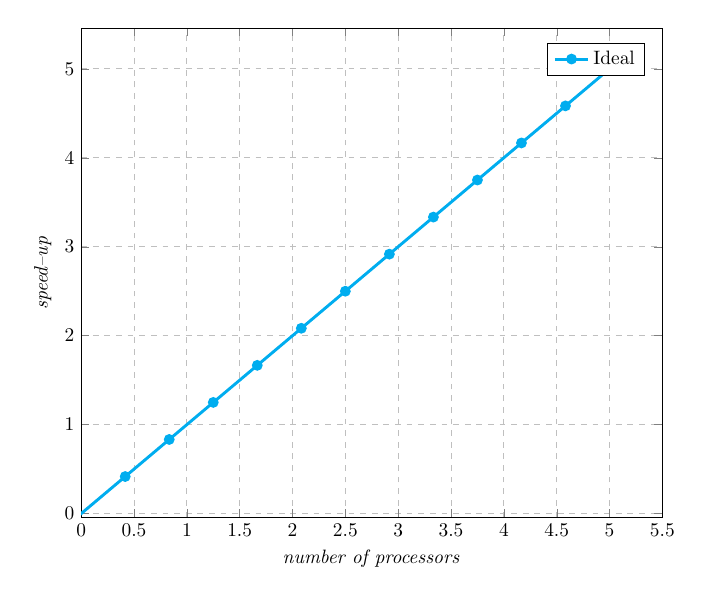
\begin{tikzpicture}[scale=0.7]	 	
		\pgfplotsset{width=\textwidth}
			\begin{axis}[
				xlabel = {\emph{number of processors}},
				ylabel = {\emph{speed--up}},
				%ymin = -1, ymax = 1,
				xmin = 0,% xmax = 13,
				%minor y tick num = 1,
				ymajorgrids=true,
				xmajorgrids=true,
				grid style=dashed,
				legend pos=north east
				]
				\addplot[mark=*, cyan, line width = 1.5pt] {x};
				\addlegendentryexpanded{Ideal};
				\addcustomplot{others/performance/crank-nicolson-parallel-final.csv}{red}{2}{Actual}
			\end{axis}
		\end{tikzpicture}
		\caption{Speed-up of Crank-Nicolson numerical method.}
		\label{fig:speedup:crank-nicolson}
	\end{figure}
	Maximum \gls{speed-up} for Crank-Nicolson schema presented in Figure \ref{fig:speedup:crank-nicolson} is reached for $10$ processors giving $2.52$. Performance of this parallelization if very poor reaching \gls{efficiency} equal to $25.2$. The \gls{speed-up} is bounded very fast, probably due to forward and backward substitution calculated in quasi serial way at the end of each iteration. This scheme also introduces the highest amount of data exchange (Figure \ref{fig:visualization:crank-nicolson}). Adding those facts the result is not surprising.  
	\begin{figure}[!htbp]
		\centering
		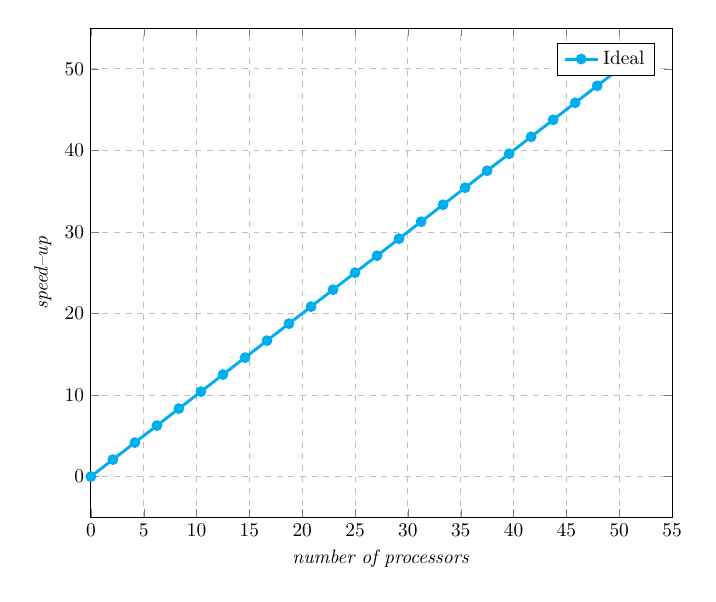
\begin{tikzpicture}[scale=0.7]	 	
			\pgfplotsset{width=\textwidth}
			\begin{axis}[
				xlabel = {\emph{number of processors}},
				ylabel = {\emph{speed--up}},
				%ymin = -1, ymax = 1,
				xmin = 0, %xmax = 13,
				%minor y tick num = 1,
				ymajorgrids=true,
				xmajorgrids=true,
				grid style=dashed,
				legend pos=north east
				]
				\addplot[domain=0:50,mark=*, cyan, line width = 1.5pt] {x};
				\addlegendentryexpanded{Ideal};
				\addcustomplot{others/performance/explicit-upwind-parallel-final.csv}{orange}{2}{Actual}
			\end{axis}
		\end{tikzpicture}
		\caption{Speed-up of Explicit Upwind numerical method.}
		\label{fig:speedup:explicit-upwind}
	\end{figure}
	Calculations in explicit upwind scheme are performed simultaneously with very low \gls{computation-to-communication-ratio}. Produced result is the best comparing to the other discussed schemes. Small dispersion (rapid growth) from the linear order can be noticed in Figure \ref{fig:speedup:explicit-upwind} between $44$ and $48$ processor. It is very hard to identify why anomaly occurred, probably it is due to memory hierarchy and caching. Maximum \gls{speed-up} is equal $33.77$ for $52$ processors. The performance for this parallel algorithm is very scalable.
	\begin{figure}[!htbp]
		\centering
		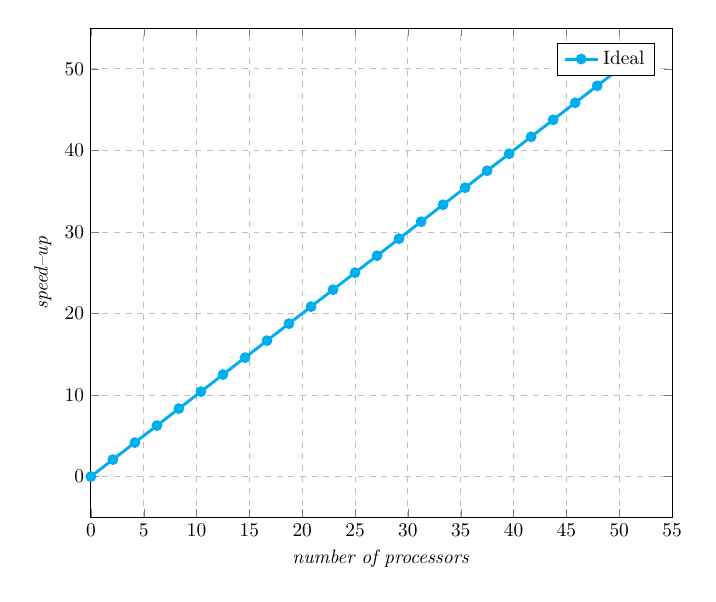
\begin{tikzpicture}[scale=0.7]	 	
		\pgfplotsset{width=\textwidth}
			\begin{axis}[
				xlabel = {\emph{number of processors}},
				ylabel = {\emph{speed--up}},
				%ymin = -1, ymax = 1,
				xmin = 0,% xmax = 13,
				%minor y tick num = 1,
				ymajorgrids=true,
				xmajorgrids=true,
				grid style=dashed,
				legend pos=north east
				]
				\addplot[domain=0:50, mark=*, cyan, line width = 1.5pt] {x};
				\addlegendentryexpanded{Ideal};
				\addcustomplot{others/performance/implicit-upwind-parallel-final.csv}{magenta}{2}{Actual}
			\end{axis}
		\end{tikzpicture}
		\caption{Speed-up of Implicit Upwind numerical method.}
		\label{fig:speedup:implcit-upwind}
	\end{figure}
	Almost classic linear growth of \gls{speed-up} is shown in Figure \ref{fig:speedup:implcit-upwind} reaching $33.14$ for $128$ processors. Due to very long queues further test cannot be performed for this scheme. Comparing to the explicit upwind slope of the \gls{speed-up} line is smaller. Fact that processors have to send a new solution to the next one cause a standby time and is a reason of slow \gls{speed-up} increase. 
	
	None of the discussed schemes was close to the ideal \gls{speed-up}, although the largest one is performed by explicit upwind scheme.